\chapter{Further Material}

\section{Data and Methods}{
	\subsection{GDD}\label{app:gdd_examples}
		\cite{baileyUsingGrowingDegree2018} tabulates the corresponding GDD for each stage of wheat.
		
		% \begin{table}[H]
			% \centering
			% \small
			\begin{tabular}{p{0.22\linewidth} p{0.6\linewidth}  p{0.13\linewidth}} 
				\toprule
				Stage  & Description    & GDD \\
				\hline Emergence & Leaf tip just emerging from above-ground coleoptyle. & $125-160$ \\
				\hline Leaf development & Two leaves unfolded. & $169-208$ \\
				\hline Tillering & First tiller visible  & $369-421$ \\
				\hline Stem elongation & First node detectable. & $592-659$ \\
				\hline Anthesis & Flowering commences; first anthers of cereals are visible. & $807-901$ \\
				\hline Seed fill & Seed fill begins. Caryopsis of cereals watery ripe (first grains have reached half of their final size). & $1068-1174$ \\
				\hline Dough stage & Soft dough stage, grain contents soft but dry, fingernail impression does not hold. & $1434-1556$ \\
				\hline Maturity complete & Grain is fully mature and drydown begins. Ready for harvest when dry. & $1538-1665$ \\
				\bottomrule
			\end{tabular}
		% \end{table}
}


\section{Interpolation}
\begin{my_figure}[H]{width=1\textwidth}{interpol/2x3_loess_robust}
	\caption[The LOESS smoother robustification.]{The LOESS smoother \RobItPlot}
	\label{fig:interpol/2x3_loess_robust}
\end{my_figure}

\begin{my_figure}[H]{width=1\textwidth}{interpol/2x3_B-Splines_robust}
	\caption[B-splines robustification.]{B-splines \RobItPlot}
	\label{fig:interpol/2x3_B-Splines_robust}
\end{my_figure}

\begin{my_figure}[H]{width=1\textwidth}{interpol/2x3_DL_robust}
	\caption[A Double Logistic curve robustification.]{A Double Logistic curve \RobItPlot}
	\label{fig:interpol/2x3_DL_robust}
\end{my_figure}

% \subsection{Skewness of LOOCV residuals}
% \begin{my_figure}[h]{width=0.6\textwidth}{interpol/res_cv}
% 	\caption{XXX caption XXX}
% 	\label{fig:interpol/res_cv}
% \end{my_figure}


\section{NDVI correction}

% step_plot/2017-201_ndvi.pdf 
% step_plot/2017-202_itpl.pdf 
% step_plot/2017-203_itpl_rew.pdf 
% step_plot/2017-204_ndvi_scl.pdf 
% step_plot/2017-205_show_res.pdf 
% step_plot/2017-206_corr.pdf 
% step_plot/2017-207_uncert.pdf 
% step_plot/2017-208_corr_itpl_rew.pdf

\begin{figure}[H]
	% \vspace{-15pt}
	% \centering
	% \begin{subfigure}[b]{0.42\textwidth}
	% 	\centering
	% 	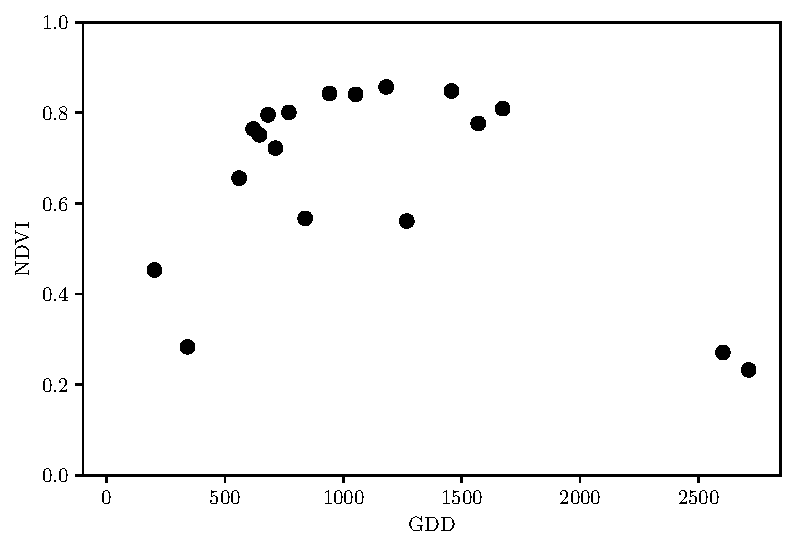
\includegraphics[width=\textwidth]{step_plot/2017-201_ndvi.pdf}
	% 	\vspace{-20pt}
	% 	\caption[NDVI {TS} with SCL45]%
	% 	{{\footnotesize NDVI {TS} with SCL45}}    
	% 	\label{fig:step_plot/2017-201_ndvi.pdf}
	% \end{subfigure}
	% \hfill
	
	\vskip\baselineskip
	\begin{subfigure}[b]{0.42\textwidth}  
		\centering 
		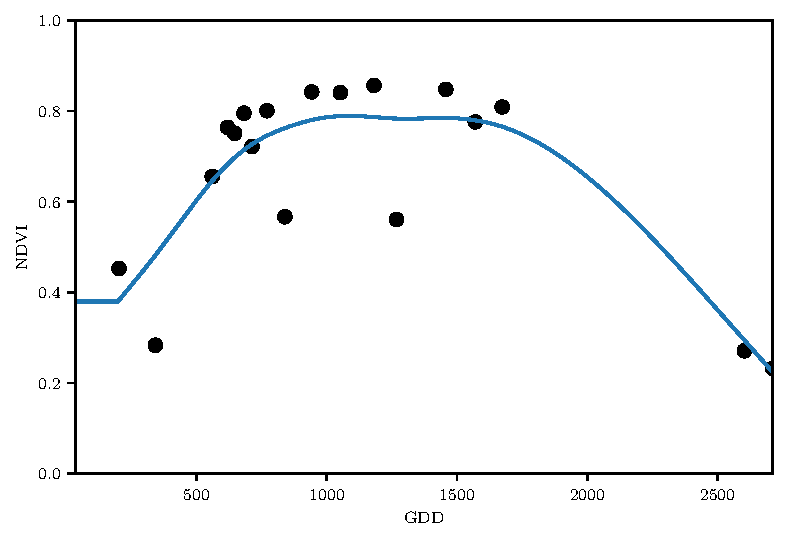
\includegraphics[width=\textwidth]{step_plot/2017-202_itpl.pdf}
		\vspace{-20pt}
		\caption[Interpolation via SS (only SCL45)]%
		{{\footnotesize Interpolation via SS (only SCL45)}}    
		\label{fig:step_plot/2017-202_itpl.pdf}
	\end{subfigure}
	% \begin{subfigure}[b]{0.42\textwidth}   
	% 	\centering 
	% 	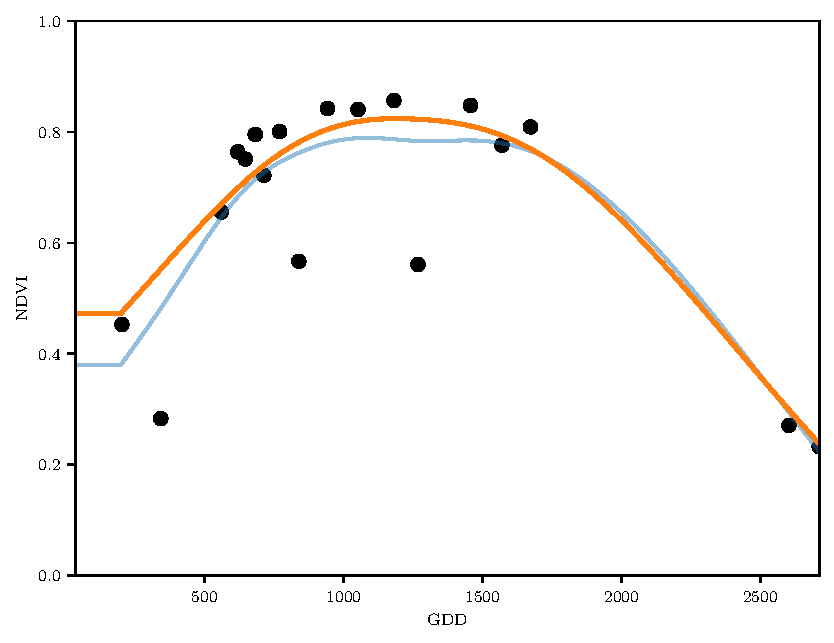
\includegraphics[width=\textwidth]{step_plot/2017-203_itpl_rew.pdf}
	% 	\vspace{-20pt}
	% 	\caption[Robustly reweighted fit]%
	% 	{{\footnotesize Robustly reweighted fit}}    
	% 	\label{fig:step_plot/2017-203_itpl_rew.pdf}
	% \end{subfigure}
	\hfill
	\begin{subfigure}[b]{0.42\textwidth}   
		\centering 
		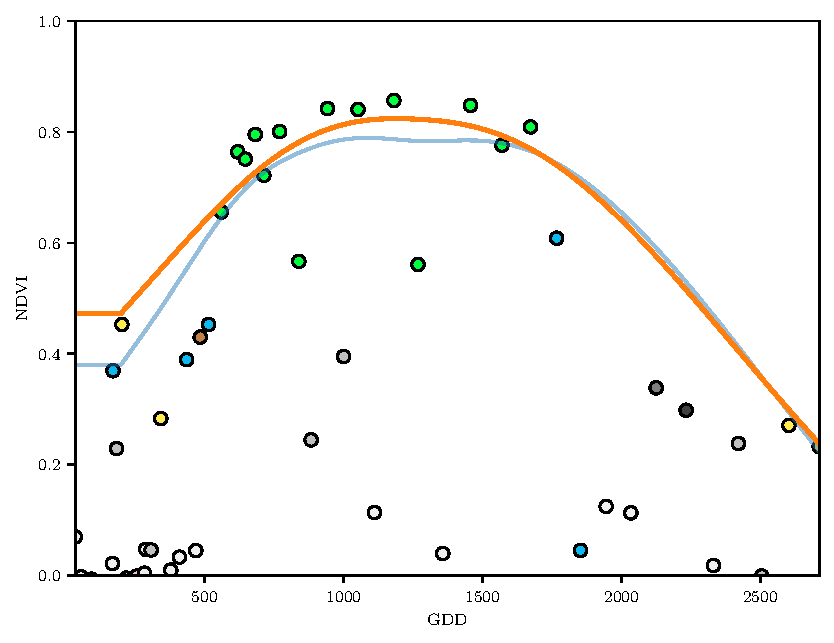
\includegraphics[width=\textwidth]{step_plot/2017-204_ndvi_scl.pdf}
		\vspace{-20pt}
		\caption[Now also consider other SCL-classes]%
		{\footnotesize Now also consider other SCL-classes}    
		\label{fig:step_plot/2017-204_ndvi_scl.pdf}
	\end{subfigure}

	\vskip\baselineskip
	\begin{subfigure}[b]{0.42\textwidth}   
		\centering 
		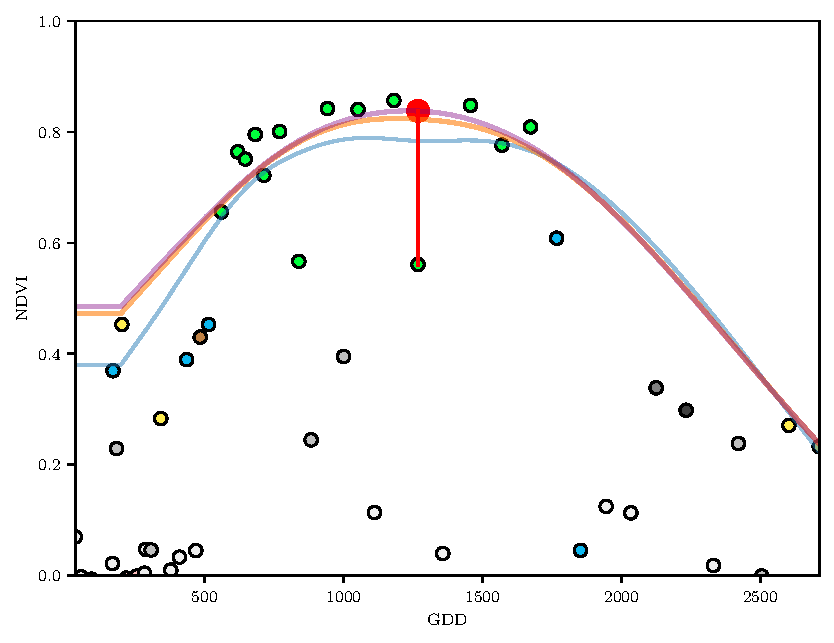
\includegraphics[width=\textwidth]{step_plot/2017-205_show_res.pdf}
		\vspace{-20pt}
		\caption[OOB estim. for each point using SCL45]%
		{{\footnotesize OOB estim. for each point using SCL45}}    
		\label{fig:step_plot/2017-205_show_res.pdf}
	\end{subfigure}
	\hfill
	\begin{subfigure}[b]{0.42\textwidth}   
		\centering 
		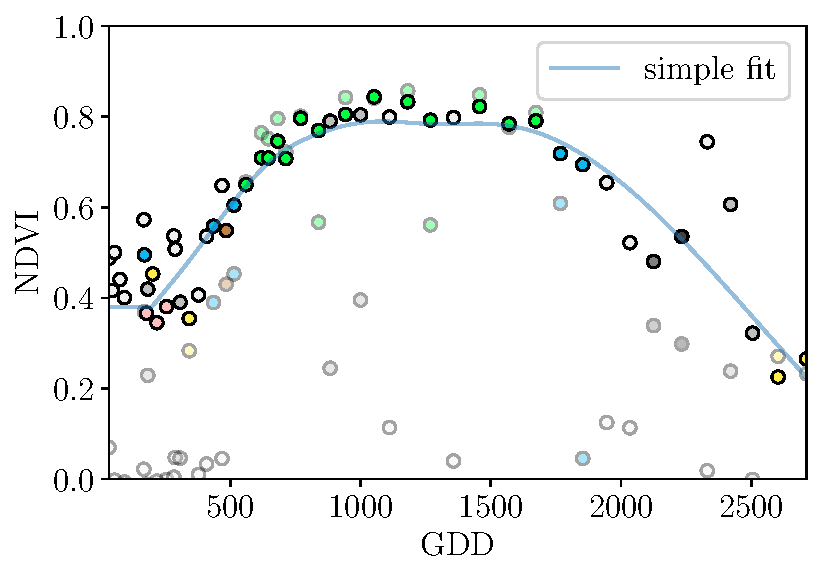
\includegraphics[width=\textwidth]{step_plot/2017-206_corr.pdf}
		\vspace{-20pt}
		\caption[Correct NDVI]%
		{\footnotesize Correct NDVI}    
		\label{fig:step_plot/2017-206_corr.pdf}
	\end{subfigure}

	\vskip\baselineskip
	\begin{subfigure}[b]{0.42\textwidth}   
		\centering 
		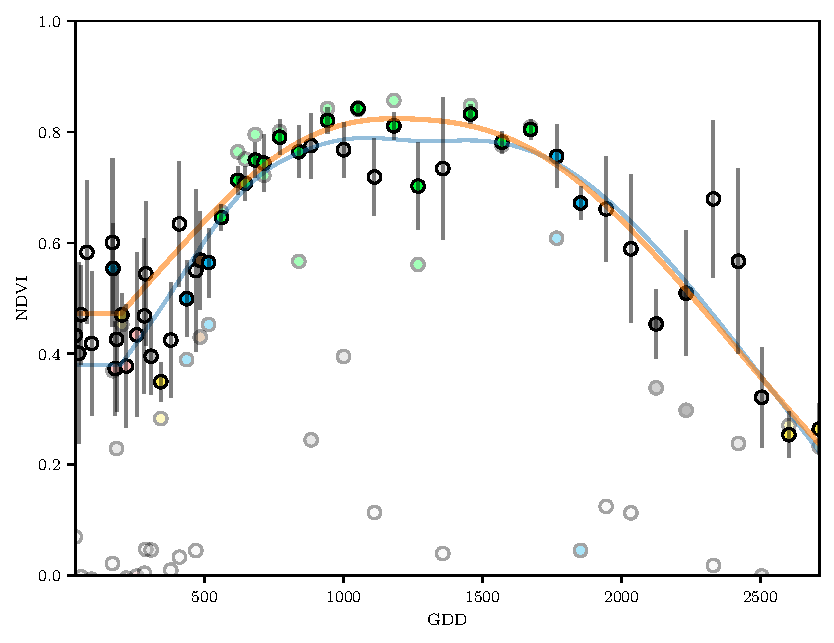
\includegraphics[width=\textwidth]{step_plot/2017-207_uncert.pdf}
		\vspace{-20pt}
		\caption[Estimate absolute errors]%
		{{\footnotesize Estimate absolute errors via statistical model}}    
		\label{fig:step_plot/2017-207_uncert.pdf}
	\end{subfigure}
	\hfill
	\begin{subfigure}[b]{0.42\textwidth}   
		\centering 
		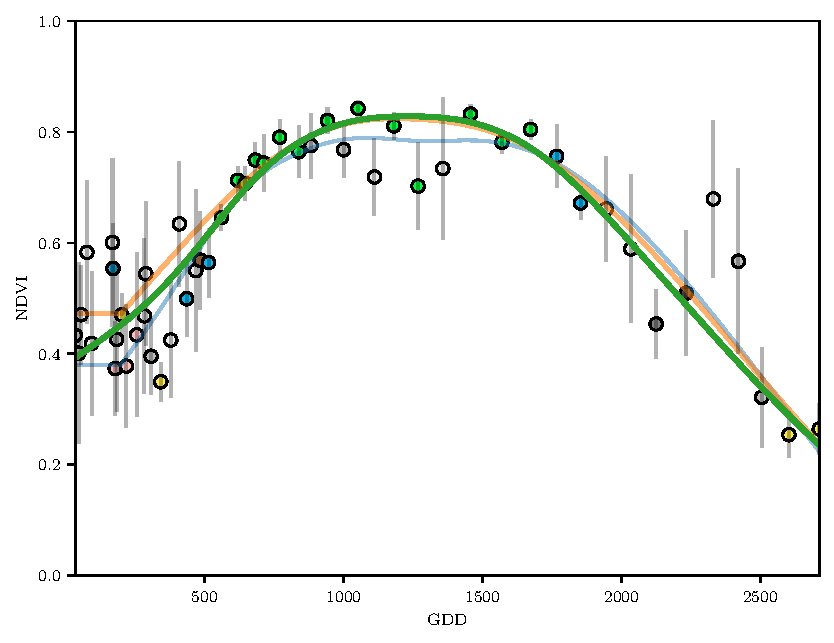
\includegraphics[width=\textwidth]{step_plot/2017-208_corr_itpl_rew.pdf}
		\vspace{-20pt}
		\caption[Interpolation (SS) on weights derived from uncertainties.]%
		{\footnotesize Robust interpolation on weights derived from uncertainties.}    
		\label{fig:step_plot/2017-208_corr_itpl_rew.pdf}
	\end{subfigure}
	\caption[Stepwise illustration of robust NDVI-Correction.]{Stepwise illustration of robust NDVI-Correction. For the color encoding of the SCL classes we refer to table~\ref{tab:satelite/scl_classes}.}
	\label{fig:step_plot_ndvi_corr}
\end{figure}


\begin{table}[H]
	\begin{center}
		\caption{Non-relative RMSE for yield prediction in [t/ha] (cf. table \ref{tab:methods_vs_yieldprediction_relative})}
		\small
		\begin{tabular}{lrrrrrrr}
\toprule
 & RF & OLS-SCL & OLS-all & MARS & GAM & LASSO & no-correction \\
\midrule
ss & {\cellcolor[HTML]{000000}} \color[HTML]{F1F1F1} 1.144 & {\cellcolor[HTML]{F1F1F1}} \color[HTML]{000000} 1.033 & {\cellcolor[HTML]{CACACA}} \color[HTML]{000000} 1.051 & {\cellcolor[HTML]{DDDDDD}} \color[HTML]{000000} 1.042 & {\cellcolor[HTML]{D4D4D4}} \color[HTML]{000000} 1.046 & {\cellcolor[HTML]{DDDDDD}} \color[HTML]{000000} 1.042 & {\cellcolor[HTML]{6A6A6A}} \color[HTML]{F1F1F1} 1.095 \\
dl & {\cellcolor[HTML]{222222}} \color[HTML]{F1F1F1} 1.150 & {\cellcolor[HTML]{ADADAD}} \color[HTML]{000000} 1.115 & {\cellcolor[HTML]{A7A7A7}} \color[HTML]{F1F1F1} 1.116 & {\cellcolor[HTML]{A7A7A7}} \color[HTML]{F1F1F1} 1.116 & {\cellcolor[HTML]{F1F1F1}} \color[HTML]{000000} 1.097 & {\cellcolor[HTML]{EDEDED}} \color[HTML]{000000} 1.098 & {\cellcolor[HTML]{000000}} \color[HTML]{F1F1F1} 1.159 \\
ss-rob & {\cellcolor[HTML]{000000}} \color[HTML]{F1F1F1} 1.144 & {\cellcolor[HTML]{F1F1F1}} \color[HTML]{000000} 1.054 & {\cellcolor[HTML]{A2A2A2}} \color[HTML]{F1F1F1} 1.084 & {\cellcolor[HTML]{878787}} \color[HTML]{F1F1F1} 1.094 & {\cellcolor[HTML]{C3C3C3}} \color[HTML]{000000} 1.072 & {\cellcolor[HTML]{C5C5C5}} \color[HTML]{000000} 1.071 & {\cellcolor[HTML]{8F8F8F}} \color[HTML]{F1F1F1} 1.091 \\
dl-rob & {\cellcolor[HTML]{000000}} \color[HTML]{F1F1F1} 1.159 & {\cellcolor[HTML]{4E4E4E}} \color[HTML]{F1F1F1} 1.128 & {\cellcolor[HTML]{696969}} \color[HTML]{F1F1F1} 1.117 & {\cellcolor[HTML]{F1F1F1}} \color[HTML]{000000} 1.064 & {\cellcolor[HTML]{A8A8A8}} \color[HTML]{F1F1F1} 1.093 & {\cellcolor[HTML]{888888}} \color[HTML]{F1F1F1} 1.105 & {\cellcolor[HTML]{060606}} \color[HTML]{F1F1F1} 1.156 \\
\bottomrule
\end{tabular}

		\label{tab:methods_vs_yieldprediction}
		\normalsize
	\end{center}
\end{table}


\begin{table}[H]
	\begin{center}
		\caption{Coefficient of determination (R\textsuperscript{2}) of yield prediction (cf. table \ref{tab:methods_vs_yieldprediction_relative})}
		\small
		\begin{tabular}{lrrrrrrr}
\toprule
 & RF & OLS-SCL & OLS-all & MARS & GAM & LASSO & no-correction \\
\midrule
ss & {\cellcolor[HTML]{F1F1F1}} \color[HTML]{000000} 0.431 & {\cellcolor[HTML]{000000}} \color[HTML]{F1F1F1} 0.486 & {\cellcolor[HTML]{272727}} \color[HTML]{F1F1F1} 0.477 & {\cellcolor[HTML]{141414}} \color[HTML]{F1F1F1} 0.481 & {\cellcolor[HTML]{1C1C1C}} \color[HTML]{F1F1F1} 0.479 & {\cellcolor[HTML]{141414}} \color[HTML]{F1F1F1} 0.481 & {\cellcolor[HTML]{878787}} \color[HTML]{F1F1F1} 0.455 \\
dl & {\cellcolor[HTML]{CFCFCF}} \color[HTML]{000000} 0.427 & {\cellcolor[HTML]{444444}} \color[HTML]{F1F1F1} 0.445 & {\cellcolor[HTML]{4A4A4A}} \color[HTML]{F1F1F1} 0.444 & {\cellcolor[HTML]{4A4A4A}} \color[HTML]{F1F1F1} 0.444 & {\cellcolor[HTML]{000000}} \color[HTML]{F1F1F1} 0.454 & {\cellcolor[HTML]{040404}} \color[HTML]{F1F1F1} 0.453 & {\cellcolor[HTML]{F1F1F1}} \color[HTML]{000000} 0.423 \\
ss-rob & {\cellcolor[HTML]{F1F1F1}} \color[HTML]{000000} 0.431 & {\cellcolor[HTML]{000000}} \color[HTML]{F1F1F1} 0.475 & {\cellcolor[HTML]{4E4E4E}} \color[HTML]{F1F1F1} 0.461 & {\cellcolor[HTML]{6A6A6A}} \color[HTML]{F1F1F1} 0.456 & {\cellcolor[HTML]{2D2D2D}} \color[HTML]{F1F1F1} 0.467 & {\cellcolor[HTML]{2B2B2B}} \color[HTML]{F1F1F1} 0.467 & {\cellcolor[HTML]{616161}} \color[HTML]{F1F1F1} 0.457 \\
dl-rob & {\cellcolor[HTML]{F1F1F1}} \color[HTML]{000000} 0.423 & {\cellcolor[HTML]{A2A2A2}} \color[HTML]{F1F1F1} 0.439 & {\cellcolor[HTML]{888888}} \color[HTML]{F1F1F1} 0.444 & {\cellcolor[HTML]{000000}} \color[HTML]{F1F1F1} 0.470 & {\cellcolor[HTML]{494949}} \color[HTML]{F1F1F1} 0.456 & {\cellcolor[HTML]{696969}} \color[HTML]{F1F1F1} 0.450 & {\cellcolor[HTML]{EBEBEB}} \color[HTML]{000000} 0.424 \\
\bottomrule
\end{tabular}

		\label{tab:methods_vs_yieldprediction_r2}
		\normalsize
	\end{center}
\end{table}

\subsection{OLS\textsuperscript{SCL} Model Outputs}\label{app:ols-scl-summary}
\lstinputlisting[title= R Summary of the NDVI correction model (cf. equation~\refeq{eq:corr_lm})]{tex/chapters/misc/lm_scl.txt}
\lstinputlisting[title= R Summary of the NDVI correction model (cf. equation~\refeq{eq:corr_lm_res})]{tex/chapters/misc/lm_scl_res.txt}


\todo[inline]{check quantile und LOOCV definitions}
\todo[inline]{figure spacing (caption zu nah dran --- manuell vspace einfügen wo nötig)}
